\documentclass[a4paper,14pt]{scrreprt}
\usepackage[T1]{fontenc}
\usepackage[utf8]{inputenc}
\usepackage[ngerman]{babel}
\usepackage[table]{xcolor}% http://ctan.org/pkg/xcolor
\usepackage{tabu}
\usepackage{graphicx}
\usepackage{lmodern}
\usepackage{hyperref}
\usepackage{listings}
\usepackage{geometry}
\geometry{verbose,a4paper,tmargin=22mm,bmargin=45mm,lmargin=30mm,rmargin=30mm}

\begin{document}


%\titlehead{Kopf} %Optionale Kopfzeile
\author{Alexander Rieppel} %Zwei Autoren
\title{Java Virtual Machine} %Titel/Thema
\subject{FT-Ausarbeitung} %Fach
\subtitle{Bestandteile und Funktionsweise} %Genaueres Thema, Optional
\date{\today} %Datum
\publishers{5AHITT} %Klasse

\maketitle
\tableofcontents
\bibliographystyle{alphadin} 

\chapter{Einführung}
Die Java Virtual Machine (JVM) wird innerhalb der Java Laufzeitumgebung (JRE) angeboten, welche für die Ausführung des Byte-Codes von Java-Programmen verantwortlich ist. Im Normalfall wird jedes gestartete Programm in seiner eigenen virtuellen Umgebung ausgeführt. Den restlichen Teil der JRE stellen die Java-Klassenbibliotheken dar. Die JVM dient als Schnittstelle zwischen Maschine und Betriebssystem und ist für Microsoft Windows, Linux, Mac OS X und andere  Plattformen verfügbar. 
\begin{figure}[h!]
\centering
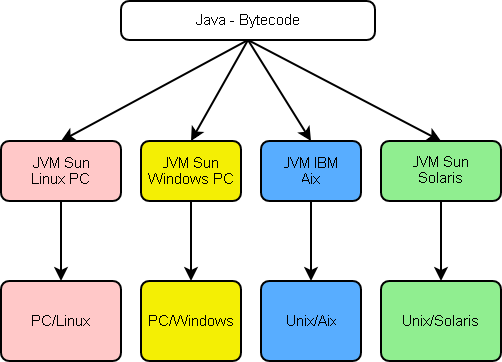
\includegraphics[width=0.8\linewidth]{./Java-jvm}
\caption[Java Virtual Machine als Schnittstelle]{Java Virtual Machine als Schnittstelle}
\label{fig:Java-jvm}
\end{figure}\newpage
Die JVM besteht aus folgenden Teilen:
\begin{itemize}
\item Classloader
\item Garbage Collector
\item Execution Engine
\end{itemize}
\section{Funktionsweise}
Die Java Virtual Machine ist dazu da, um den Byte-Code der vom Java-Compiler erzeugt wurde, auf der jeweiligen Plattform auf der er ausgeführt werden soll ausführbar zu machen. Dazu werden die verschiedenen Byte-Code Dateien die erzeugt wurden (zu erkennen an Dateieindung "'class"') während der Laufzeit in die, vom jeweiligen Rechner verstandene Maschinensprache übersetzt. Die JVM arbeitet im Prinzip wie ein Interpreter, allerdings um einiges schneller, da nicht mehr auf Syntaxfehler geachtet werden muss. 
\section{Sicherheit}
Die JVM ist neben der Plattformunabhängigkeit auch für ein gewisses Maß an Sicherheit verantwortlich. Sie überwacht während der Laufzeit die Ausführung der Programme und verhindert Pufferüberläufe, welche zu unvorhersehbarem Verhalten wie zum Beispiel ein Absturz des Programmes führen können. Diese Überwachung ist allerdings ziemlich einfach, da Pointer von Java nur implizit unterstützt werden.
\section{Optimierungsverfahren}
Um die Performance von Java-Programmen zu erhöhen, setzen die meisten Java-VMs sogenannte JIT-Compiler (Just-In-Time-Compiler oder JITC) ein, die unmittelbar während des Programmablaufs den Bytecode "'genau zur rechten Zeit"' in Maschinensprache übersetzen. Eine Weiterentwicklung ist der Hotspot-Optimizer, welcher dynamische Optimierung anbietet.
\subsection{Dynamische Optimierung}
Oft ist zum Zeitpunkt der Kompilierung nicht bekannt, welche konkreten Eingaben eine Software verarbeiten muss. Demnach muss die Software mit allen Arten von Eingaben zurechtkommen. Die Eingabe wird deshalb in Variablen gespeichert. Nach dem Start des Programms werden jedoch viele Variablen nicht mehr geändert. Folglich sind diese - von einem Zeitpunkt kurz nach dem Start an - Konstanten. Wird nun erst nach diesem Zeitpunkt die Software für die System-Architektur kompiliert (dies ist bei Java Hotspot der Fall), so können diese Konstanten berücksichtigt werden. Bestimmte Verzweigungen, die nur von solchen „Halbkonstanten“ abhängig sind, sind dann für immer eindeutig und stellen somit kein Risiko für eine falsche Sprungvorhersage dar. Ein solcher Programmcode kann also schneller ablaufen als zu früh compilierter Code.
\section{Implementierung in Hardware}
Ausführungen in Hardware sind Java-Prozessoren und Mikroprozessoren, die Java-Bytecode als Maschinensprache verwenden. Sie konnten sich gegen die schnelle Steigerung der Leistungsfähigkeit von Standard-PC und der JVM nicht durchsetzen.
\section{Threads}
Die Java VM schottet die in ihr laufenden Prozesse vom Betriebssystem ab (Green Threads). Sie bildet standardmäßig Java-Threads durch Threads des Betriebssystems ab und nur in Ausnahmefällen erfolgt das Thread-Management durch die Java VM. Somit ist es auch möglich, auf einem Betriebssystem, das kein Multithreading unterstützt, eine Java VM in vollem Funktionsumfang anzubieten. \\\\Die Java VM hat stets volle und standardkonforme Kontrolle über die Java-Threads, d.h. der Programmierer braucht nicht die betriebssystemspezifischen Multi-Threading/Tasking/Processing-Eigenschaften zu berücksichtigen und kann sich stets auf die JRE verlassen. Nachteil ist, dass Probleme, die von einem Thread ausgehen, seitens des Betriebssystems dem gesamten Prozess zugeordnet werden. Gängige Betriebssysteme (wie zum Beispiel Linux, Windows) erlauben Kontrolle über diese „nativen“ Threads allenfalls über Software von Drittanbietern, wie beispielsweise die mit dem JDK mitgelieferte VisualVM. Standardwerkzeuge wie zum Beispiel der Windows Taskmanager zeigen solche Threads jedoch nicht an.
\section{JVM kompatible Sprachen}
Neben Java gibt es auch andere Sprachen, die als Programmiersprachen für JVM-Programme benutzt werden können. Unter anderem folgende Sprachen können auf einer JVM laufen:
\begin{itemize}
\item Clojure, ein Lisp-Dialekt
\item Ceylon
\item Erjang, ein Erlang-Dialekt für die JVM
\item Free Pascal, das auch unter der JVM einen Großteil der Object-Pascal-Konstrukte unterstützt
\item Groovy, eine dynamisch typisierte Programmiersprache
\item JRuby, eine 100 \% Ruby-kompatible Implementierung
\item Jython (früher: JPython), ist eine reine Java-Implementierung der Programmiersprache Python
\item Scala, eine Sprache, die Eigenschaften von Java mit funktionaler Programmierung vereint
\item Kotlin, eine 2011 vorgestellte Sprache von JetBrains
\item Jill, Kahlua (LUA)
\item Rhino (JavaScript)
\item Jacl (Tcl)
\item Quercus (PHP)
\item JavaFX
\end{itemize}\cite{ullen2011}\cite{jvmEin}\cite{jvmEin1}

\chapter{Die Bestandteile der Java Virtual Machine}
\lstset{language=Java, 
   basicstyle=\small, 
   keywordstyle=\color{black}, 
   identifierstyle=, 
   commentstyle=\color{darkgray}, 
   stringstyle=\ttfamily, 
   breaklines=true, 
   numbers=left, 
   numberstyle=\small, 
   frame=single, 
   backgroundcolor=\color{white} 
}
Wie zuvor bereits erwähnt besteht die JVM aus folgenden Teilen:
\begin{itemize}
\item Classloader
\item Garbage Collector
\item Execution Engine
\end{itemize}
Auf diese wird in den folgenden Punkten genauer eingegangen.
\section{Classloader}
\subsection{Allgemeines}
Der ClassLoader konstruiert Class-Objekte aus Bytecode. Eine Klasse in Java wird durch seinen voll qualifizierten Namen UND dem ClassLoader (der ihn geladen hat) identifiziert, jedoch nicht allein durch seinen voll qualifizierten Namen. Daher ist es möglich, dass mehrere Klassen mit dem selben Namen in einer VM gleichzeitig existieren, solange sie von verschiedenen ClassLoadern geladen wurden. Zwei Klassen, die mit verschiedenen ClassLoadern geladen wurden, sind von verschiedenen Typen (inkompatibel!), selbst wenn sie von ein und dem selben *.class-file geladen wurden. Dadurch können mehrere Klassen mit den gleichen Namen gleichzeitig existieren. Sie müssen lediglich durch andere ClassLoader geladen werden. In der Praxis instantiiert man einfach immer einen neuen ClassLoader. Somit können Namen "wiederverwendet" werden:
\begin{lstlisting}
Class<?> autoClass = new MyClassLoader().loadClass("pkg.Auto");
\end{lstlisting}
java.lang.ClassLoader ist eine abstrakte Klasse. Um selbst Klassen zur Laufzeit zu laden, muss ClassLoader erweitert werden. Wenn die JVM hochfährt, lädt der SystemClassLoader alle Klassen im ClassPath. Schreibt man z.B. "new Auto()" wird der SystemClassLoader diese Klasse laden. Mit der statischen Methode ClassLoader.getSystemClassLoader() kann eine Referenz auf den SystemClassLoader erhalten werden:
\begin{lstlisting}
ClassLoader systemClassLoader = ClassLoader.getSystemClassLoader();
System.out.println(systemClassLoader); //"sun.misc.Launcher$AppClassLoader@11b86e7"
\end{lstlisting}
Liefert <Objekt>.getClass().getClassLoader() null zurück, so wurde diese Klasse vom SystemClassLoader geladen.
\subsection{Delegation}
Die ClassLoader verfolgen das Konzept der Delegation. Er hat immer einen Parent-Classloader. Wenn der ClassLoader eine Klasse laden soll, delegiert er die Aufgabe an seinen Parent. Wenn der Parent die Klasse nicht finden kann, versucht er selbst die Klasse zu laden. Der oberste Parent in der Delegationshirarchie ist der SystemClassLoader.
\begin{figure}[h!]
\centering
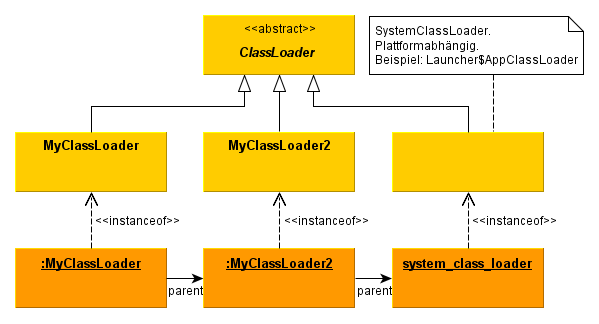
\includegraphics[width=0.8\linewidth]{./classloader-hierarchie}
\caption[Vererbungshierarchie von ClassLoader und die Parentassoziation]{Vererbungshierarchie von ClassLoader und die Parentassoziation}
\label{fig:classloader-hierarchie}
\end{figure}
\newpage
\subsection{API}
Innerhalb des Classloader-Objektes existieren einige Methoden. Eine der wichtigsten stellt die loadClass() Methode dar. Mit dieser beginnt der Prozess des eigentlichen Ladens. Die JVM lädt dabei alle Klassen, in der sie loadClass() aufruft. Im folgender Grafik wird die Funktionsweise der Defaultimplementierung geschildert.
\begin{figure}[h!]
\centering
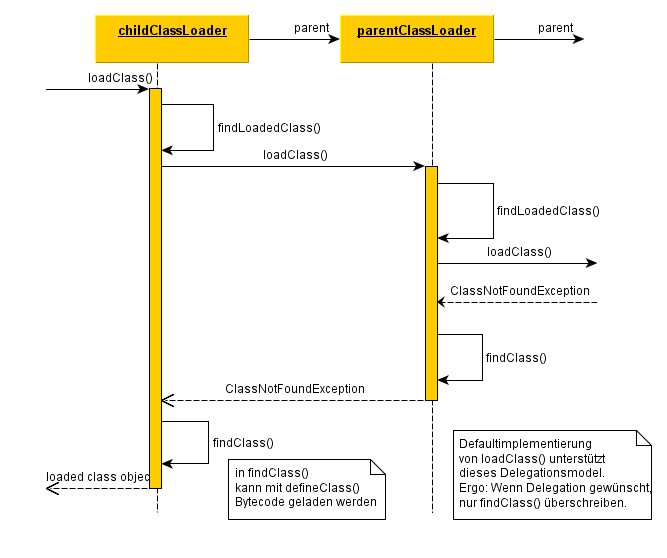
\includegraphics[width=0.8\linewidth]{./classloader-seq}
\caption[Funktionsweise von loadClass() als UML-Sequenzdiagramm]{Funktionsweise von loadClass() als Sequenzdiagramm}
\label{fig:classloader-seq}
\end{figure}
\begin{enumerate}
\item Aufruf von findLoadedClass(), um zu checken, ob die Klasse nicht bereits vom ClassLoader selbst geladen wurde. ClassLoader merken sich die Klassen, die sie selbst geladen haben. Subklassen erben dieses Verhalten.
\item Wenn keine Klasse gefunden wurde, wird loadClass() auf dem Parent-ClassLoader aufgerufen. Die Defaultimplementierung von loadClass() unterstützt somit das Delegationsmodel.
\item Wenn wieder keine Klasse gefunden wurde, wird findClass() aufgerufen. An dieser Stelle sollte man sich in seiner ClassLoader-Subklasse in den Loadingprozess einharken, wenn man das Delegationsmodell erhalten möchte. Mit der defineClass()-Methode kann hier eine Class aus Bytecode erzeugt werden.
\item Wenn einer dieser Schritte keine Class gefunden hat, wird eine ClassNotFoundException geworfen.
\end{enumerate}
\cite{jvmClass}
\section{Garbage Collector}
Garbage Collection beschreibt die automatische Speicherbereinigung um den Speicherbedarf eines Java-Programms (auch in anderen Sprachen) zu minimieren. Dies wird zur Laufzeit bewerkstelligt, wo versucht wird nicht benötigte Speicherbereiche automatisch zu erkennen und freizugeben. Der größte Vorteil von Garbage Collection ist die Vermeidung von Fehlern die bei einer manuellen Speicherverwaltung sehr leicht auftreten können. Dies geht allerdings auch mit einem gewissen Verwaltungsoverhead und oftmals nicht reproduzierbarem Verhalten der Umgebung und damit auch des Programms selbst ein her.\\\\Die Spezifikation einer JVM schreibt vor, dass in jeder Implementierung einer JVM ein Garbage Collector enthalten sein muss. Die Effizienz dieses Garbage Collectors kann großen Einfluss auf die Performance des Java Programms haben.
\subsection{Generational Garbage Collection}
Alle heutigen Garbage Collectoren in den virtuellen Maschinen für Java sind Generational Garbage Collectoren. Dieser Ansatz hat sich in der Praxis als der beste Algorithmus für Garbage Collection in Java erwiesen. Die Idee der Generational Garbage Collection besteht darin, dass man den Heap-Speicher in verschiedene Bereiche einteilt, die jeweils Objekte unterschiedlichen Alters enthalten. Mit speziellen auf das Alter der Objekte abgestimmten Algorithmen werden die jeweiligen Bereiche verwaltet und aufgeräumt.\\\\Da man in Java (anders als bspw. in C++) keine Objekte auf dem Stack anlegen kann, müssen alle Objekte auf dem Heap angelegt werden. Selbst Objekte, die nur lokal in einer Methode gebraucht werden, entstehen auf dem Heap. Die meisten dieser Objekte leben nicht lange, denn beim Verlassen der Methode werden sie bereits unerreichbar und sind damit "'tot"'.  Es gibt aber auch Heap-Objekte, die bis zum Ende der Laufzeit leben, weil sie für die gesamte Ablaufzeit der Applikation gebraucht werden, zum Beispiel final static Attribute einer Klasse.
\begin{figure}[h!]
\centering
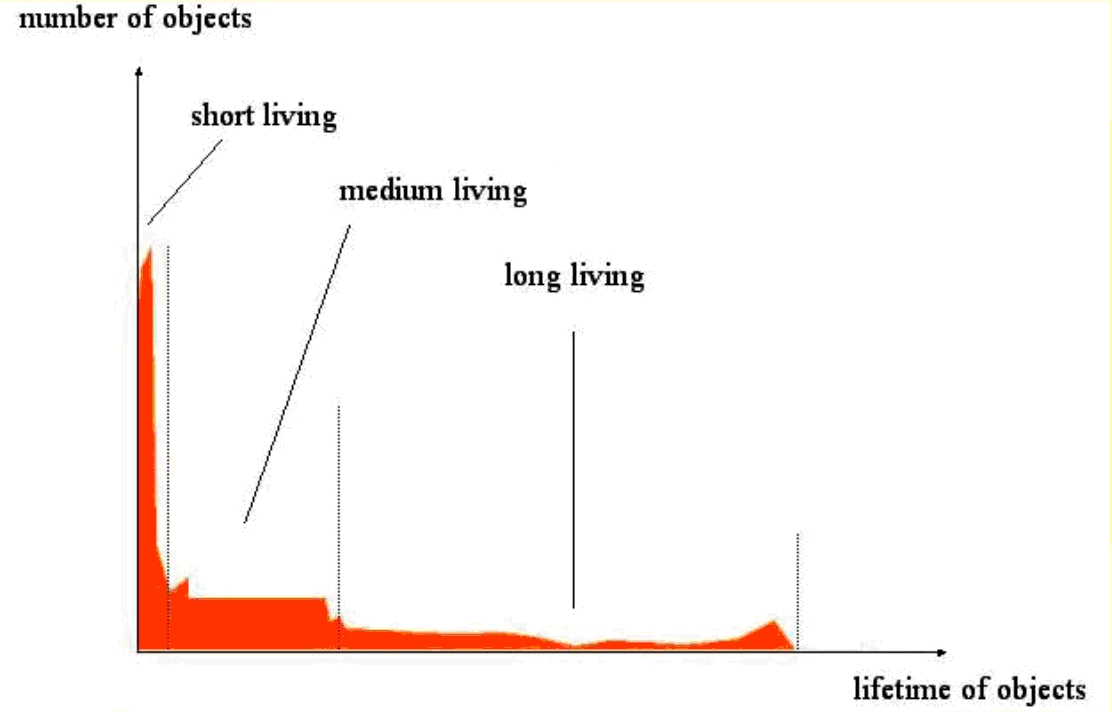
\includegraphics[width=0.8\linewidth]{./imageG8T}
\caption[Typische Objekt-Population in Java]{Typische Objekt-Population in Java}
\label{fig:imageG8T}
\end{figure}
Es gibt sehr viele Java-Objekte, die nicht sehr alt werden, und es gibt vergleichsweise wenig Objekte, die sehr lange leben.  Die Objekte mit kurzer Lebensdauer sind die, die nur innerhalb einer Methode oder manchmal nur innerhalb einer Expression gebraucht werden. Beispiele sind Iteratoren in einer Schleife oder StringBuilder fürs Zusammensetzen eines Strings. Die Objekte mit mittlerer Lebensdauer sind solche, die in nicht-stackbasierten Verarbeitungen benutzt werden. Ein Beispiel wäre der Conversational Session State einer Entity Bean. Er überlebt mehrere Methodenaufrufe und wird erst nach der Session nicht mehr gebraucht. Man beachte, die Zahl der Objekte mit mittlerer Lebensdauer ist deutlich geringer als die der kurzlebigen Objekte. Richtig alt werden nur ganz wenige Objekte. Das sind typischerweise Objekte, die schon beim Programmstart erzeugt werden und dann bis zum Ende der Anwendung in Gebrauch bleiben. Dazu gehören Thread Pools, Singletons und Objekte aus Frameworks, z.B. Servlet-Instanzen.\\\\Um den unterschiedlichen Objekt-Lebenszeiten angemessen Rechnung zu tragen, werden die Objekte verschiedenen Generationen zugeteilt. Die Generationen sind separate Bereiche des Heaps, die unterschiedlich verwaltet werden. Sie haben unterschiedliche Allokatoren und sie werden unterschiedlich oft und mit jeweils eigenen Garbage-Collection-Algorithmen aufgeräumt. Im Wesentlichen unterscheidet man zwischen einer \textbf{Young-Generation}, die häufig bereinigt wird, und einer \textbf{Old Generation}, die seltener bereinigt wird. Die Young Generation ist der Speicherbereich, in dem die neuen Objekte angelegt werden, z.B. wenn im Programm mit new Speicher angefordert wird.  Die Old Generation ist der Bereich, in den die neuen Objekte ausgelagert werden, wenn sie ein gewisses Alter erreicht haben, d.h. wenn sie eine bestimmte Anzahl von Garbage Collections überlebt haben.\\\\Dahinter steht die Beobachtung, dass von den jungen Objekten die meisten relativ schnell sterben, wie man in der Abbildung 1 gesehen hat, sodass in der Young Generation schnell viel Garbage entsteht. Da, wo viel Garbage entsteht, lohnt sich zügiges Aufräumen, weil dann rasch wieder freier Speicher zur Verfügung steht. Die Aufräumarbeiten auf die Young Generation zu beschränken, hat außerdem den Vorteil, dass nicht immer der gesamte Heap nach „toten“ Objekten durchforstet werden muss, sondern dass bereits das Aufräumen in einem Teilbereich des Heaps signifikante Mengen an Speicher freigibt.\\\\In der Old Generation lohnt sich das häufige Aufräumen nicht.  Wenn ein Objekt erst einmal mittelalt geworden ist, dann wird es mit hoher Wahrscheinlichkeit auch noch älter. In der Old Generation findet man deshalb nicht so häufig „tote“ Objekte und damit weniger Potential für die Speicherfreigabe. Also macht man die Bereinigung der Old Generation wesentlich seltener.\\\\Die Bereinigungen in der Young Generation werden als \textbf{Minor Collections} bezeichnet. Daneben gibt es die seltener durchgeführten \textbf{Major oder Full Collections}, bei denen sowohl die Young als auch die Old Generation bereinigt wird. 
\subsection{Die Heapaufteilung in einer JVM}
Seit Java 1.3 ist der Speicher in 2 Generationen (young und old) und einen Sonderbereich (perm) eingeteilt.
\begin{figure}[h!]
\centering
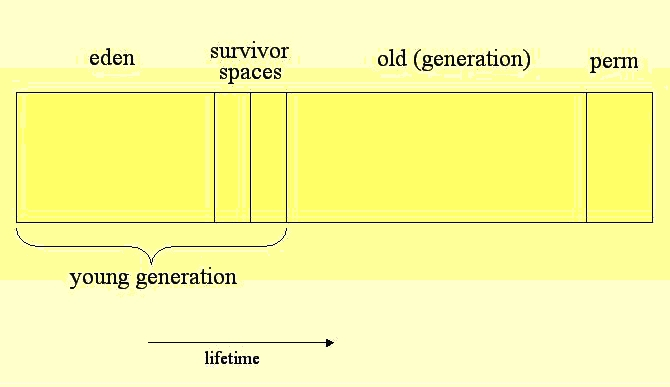
\includegraphics[width=0.8\linewidth]{./imageDD1}
\caption[Heap-Aufteilung in einer JVM]{Heap-Aufteilung in einer JVM}
\label{fig:imageDD1}
\end{figure}
\cite{jvmGarb}
\section{Execution Engine}
Die Execution-Engine ist im Prinzip die wichtigste Komponente der JVM, da diese für das eigentliche Ausführen des Java Bytecodes verantwortlich ist. In der JVM-Spezifikation ist exakt beschrieben, wie sich die Execution-Engine beim Ausführen eines Befehls verhalten soll, allerdings bleibt die Implementierung dem jeweiligen Programmierer offen. Die Execution Engine ist in der Lage, Bytecode zu interpretieren und nativen Code und Quellcode zu kompilieren. \\\\Die konkrete Implementierung kann als Softwareapplikation oder auch Hardwareversion realisiert werden. Auch sind Mischformen von beidem möglich. Code kann entweder interpretiert werden oder Just-In-Time compiliert werden. Jeder Thread der innerhalb gestartet wird stellt dabei eine eigene Laufzeitinstanz dar. \\\\Der Bytecode für die JVM besteht aus einer Sequenz von Instruktionen, wobei jede dieser Instruktionen aus dem Opcode und folgenden Operanden besteht. Der Opcode gibt der JVM an, welche Aktion von ihrer Seite ausgeführt werden soll und der Operand stellt die für die Aktionen nötigen Informationen zur Verfügung. Die Anzahl und der Typ der Operanden einer Instruktion wird durch den Opcode bestimmt. Die möglichen Befehle des Opcodes werden Befehlssatz der JVM oder Instruction Set genannt. Für das Ausführen von Bytecode durch die Execution Engine haben sich verschiedene Techniken entwickelt. Da in der Spezifikation keine Aussage über die Ausführung von Bytecode getroffen wird, stehen verschiedene Möglichkeiten zur Verfügung. Die folgenden drei Ansätze sind häufig verwendete Methoden, welche hier nun näher erläutert werden.
\subsection{Interpretation}
Die einfachste Technik zur Ausführung von Bytecode ist das Interpretationsverfahren, bei dem die Instruktionen aus dem Bytecode gelesen und ausgeführt werden. Der Code wird weder in nativen Code kompiliert, noch irgend eine Form von Codeoptimierung durchgeführt. Dieses Verfahren wird in heutigen JVMs kaum mehr eingesetzt, da das Interpretieren für heutige Anwendungen zu langsam ist. 
\subsection{Just-In-Time Kompilierung (JIT)}
Ein schnellerer und moderner Ansatz der Ausführung von Bytecode ist die Just-In-Time Kompilation, bei der Methoden bei ihrem Aufruf in nativen Code übersetzt werden. Bei diesem Verfahren besteht die Möglichkeit der Codeoptimierung, da dem Compiler zur Laufzeit bereits Informationen über das Verhalten des Codes vorliegt. Diese Technik wird in heutigen JVMs häufig eingesetzt, da sie relativ leicht zu implementieren ist. 
\subsection{Adaptive Optimierung}
Der modernste Ansatz der Codeausführung ist das Verfahren der adaptiven Optimierung, bei dem das Interpretations- und JIT-Verfahren miteinander kombiniert werden. Durch dieses Verfahren ist ein maximaler Performancegewinn möglich. Bei der adaptiven Optimierung werden die Instruktionen durch den Interpreter ausgeführt, wobei das Verhalten des Codes von der JVM beobachtet wird. Durch das beobachten ist ein Auffinden von „Hot Spots“ möglich. Hot Spots sind Codezeilen die ca. 80 – 90\% der Ausführungszeit benötigten, aber insgesamt nur 10 – 20\% vom Quellcode ausmachen. Diese „Hot Spots“ werden mit starker Optimierung in nativen Code übersetzt. 
\cite{jvmExec}
\chapter{Zusammenfassung}
Die Java Virtual Machine ist eine Umgebung in der der kompilierte Java-Code ausgeführt wird. Sie besteht aus drei großen Bestandteilen: Dem Classloader, dem Garbage Collector und der Execution Engine. \\\\Der Classloader ist für die Erstellung der Class-Objekte aus dem Byte-Code zuständig. Jedes Programm wird in der Regel von seinem eigenen Class Loader geladen. Dazu wird das Verfahren der Delegation verwendet.\\\\Der Garbage Collector ist für das "aufräumen" innerhalb der Java VM zuständig. Dies ist so zu verstehen, dass Speicherbereiche welche nicht mehr benötigt werden (also null gesetzt sind) oder generell nicht mehr erreichbar sind, aussortiert und freigegeben werden. Dazu wird das Verfahren der Generational Garbage Collection verwendet. In diesem Verfahren werden die meisten Objekte in der ersten Generation aussortiert. Alle die weiterhin gebraucht werden, werden in die nächste Generation verschoben.\\\\Die Execution Engine ist für das eigentliche Ausführen der Programme verantwortlich. Um Code auszuführen existieren drei Ansätze: Die langsame Interpretation wo keine Optimierung stattfindet und Zeile für Zeile gelesen wird. Die Just In Time Kompilierung (JIT) wo die Möglichkeit der Codeoptimierung bereits vorhanden ist. Und das kombinierte Verfahren der adaptiven Optimierung, bei der beide der erster Verfahren zum Einsatz kommen.
%\section{Java Hotspot JVM}
%\cite{jvmEin1}
\bibliography{ref}
\end{document}